\begin{figure}[H]
    \centering
    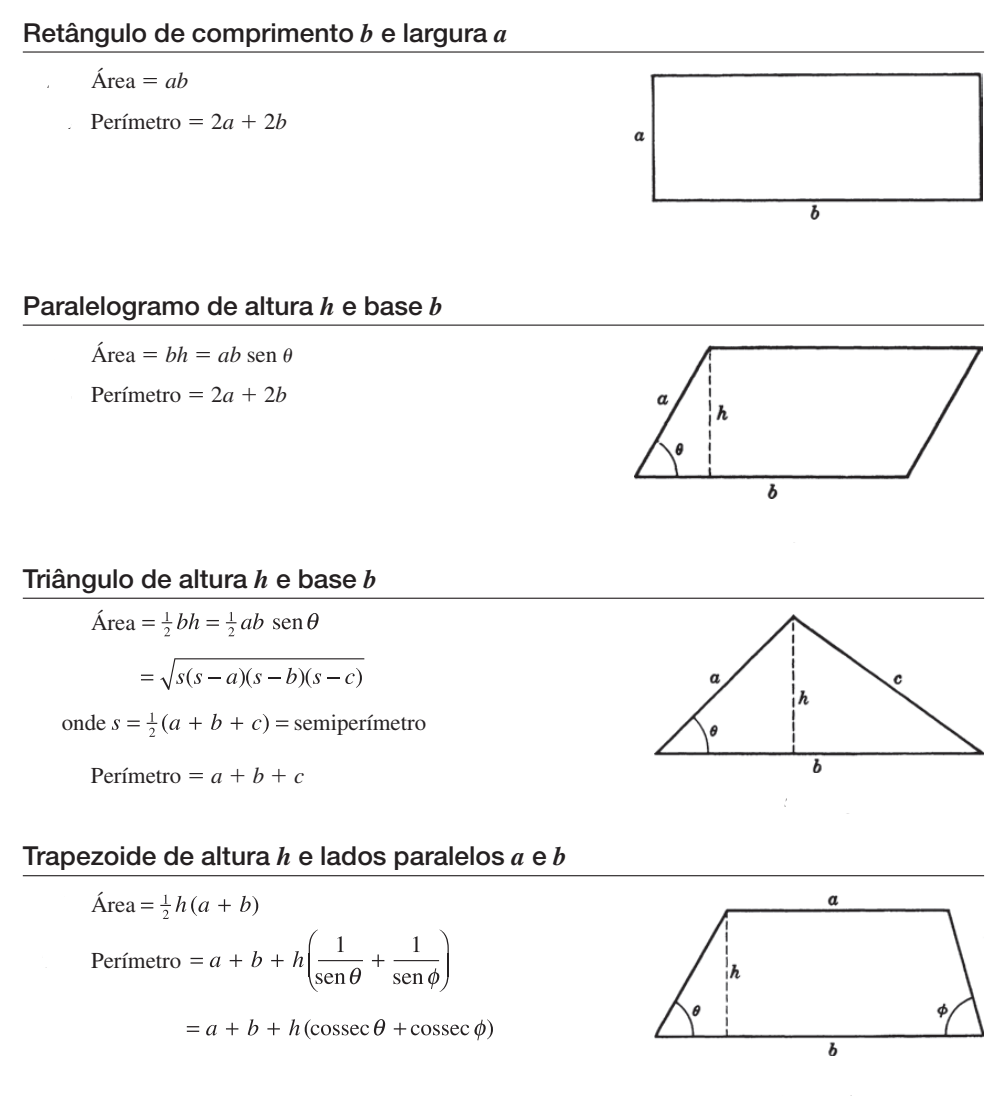
\includegraphics[width=\textwidth]{matematica/geometria/formulas1}
\end{figure}

\begin{figure}[H]
    \centering
    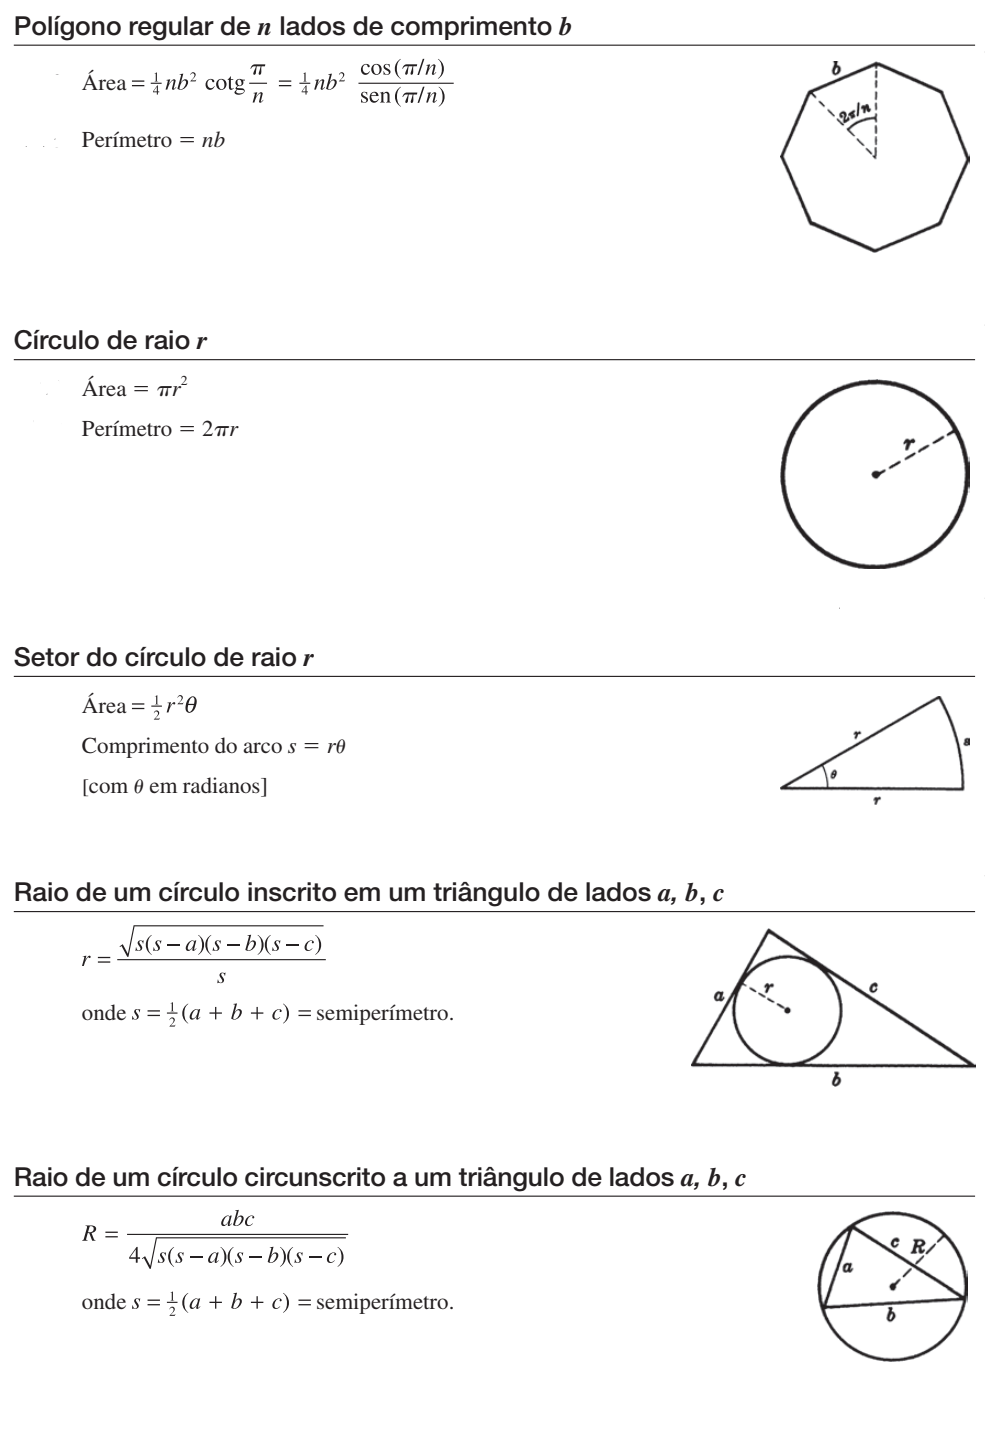
\includegraphics[width=\textwidth]{matematica/geometria/formulas2}
\end{figure}

\begin{figure}[H]
    \centering
    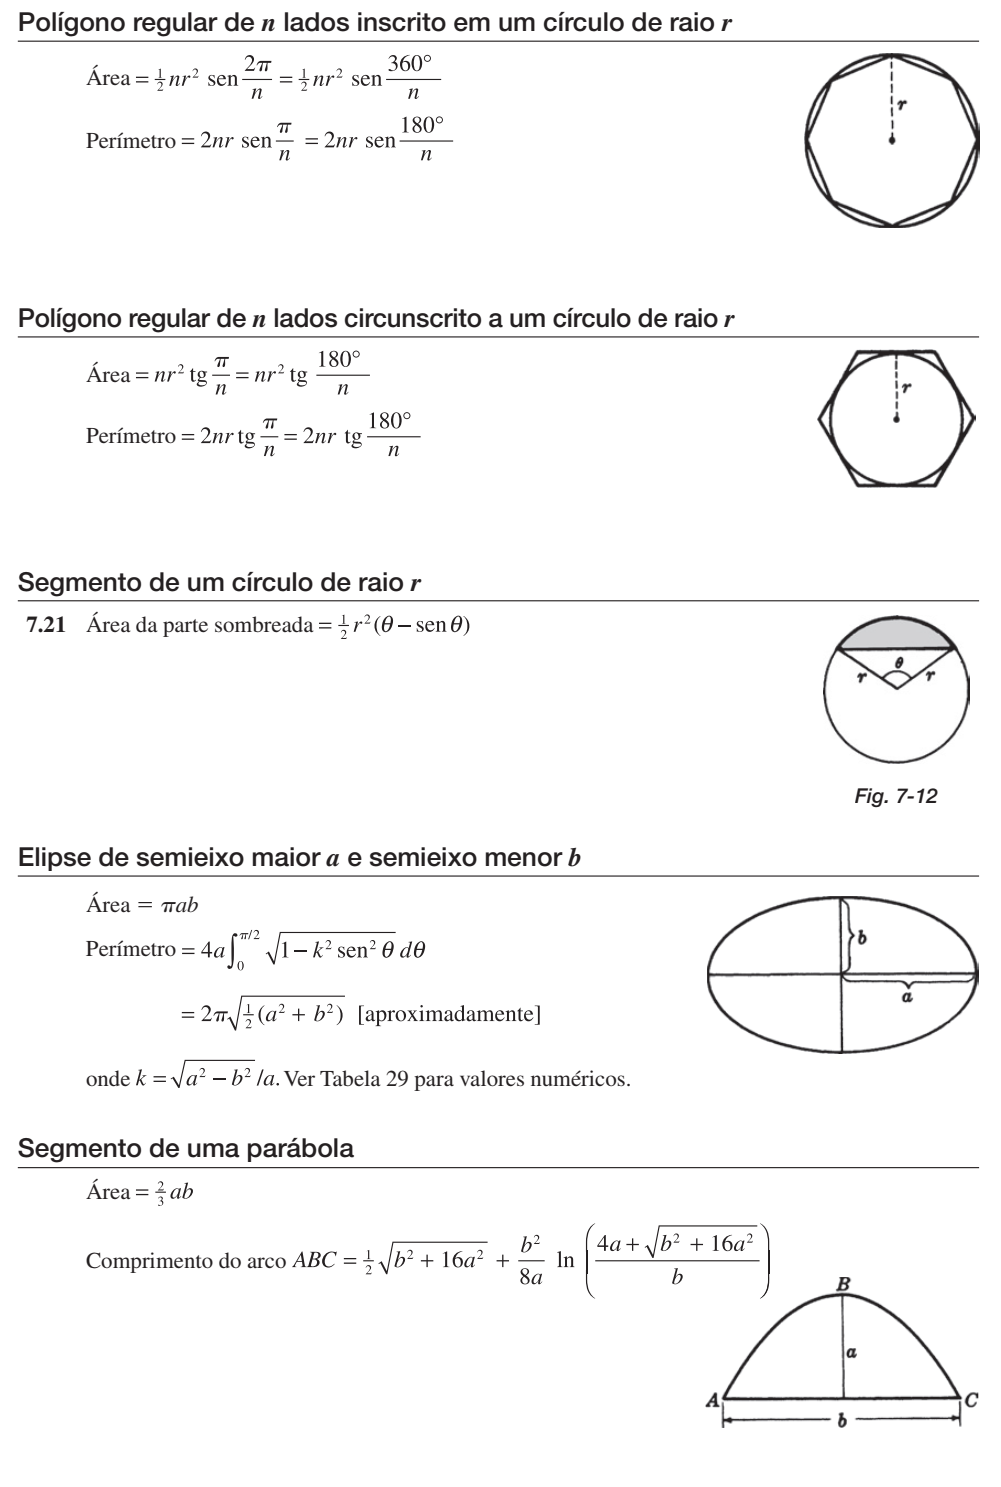
\includegraphics[width=\textwidth]{matematica/geometria/formulas3}
\end{figure}

\begin{figure}[H]
    \centering
    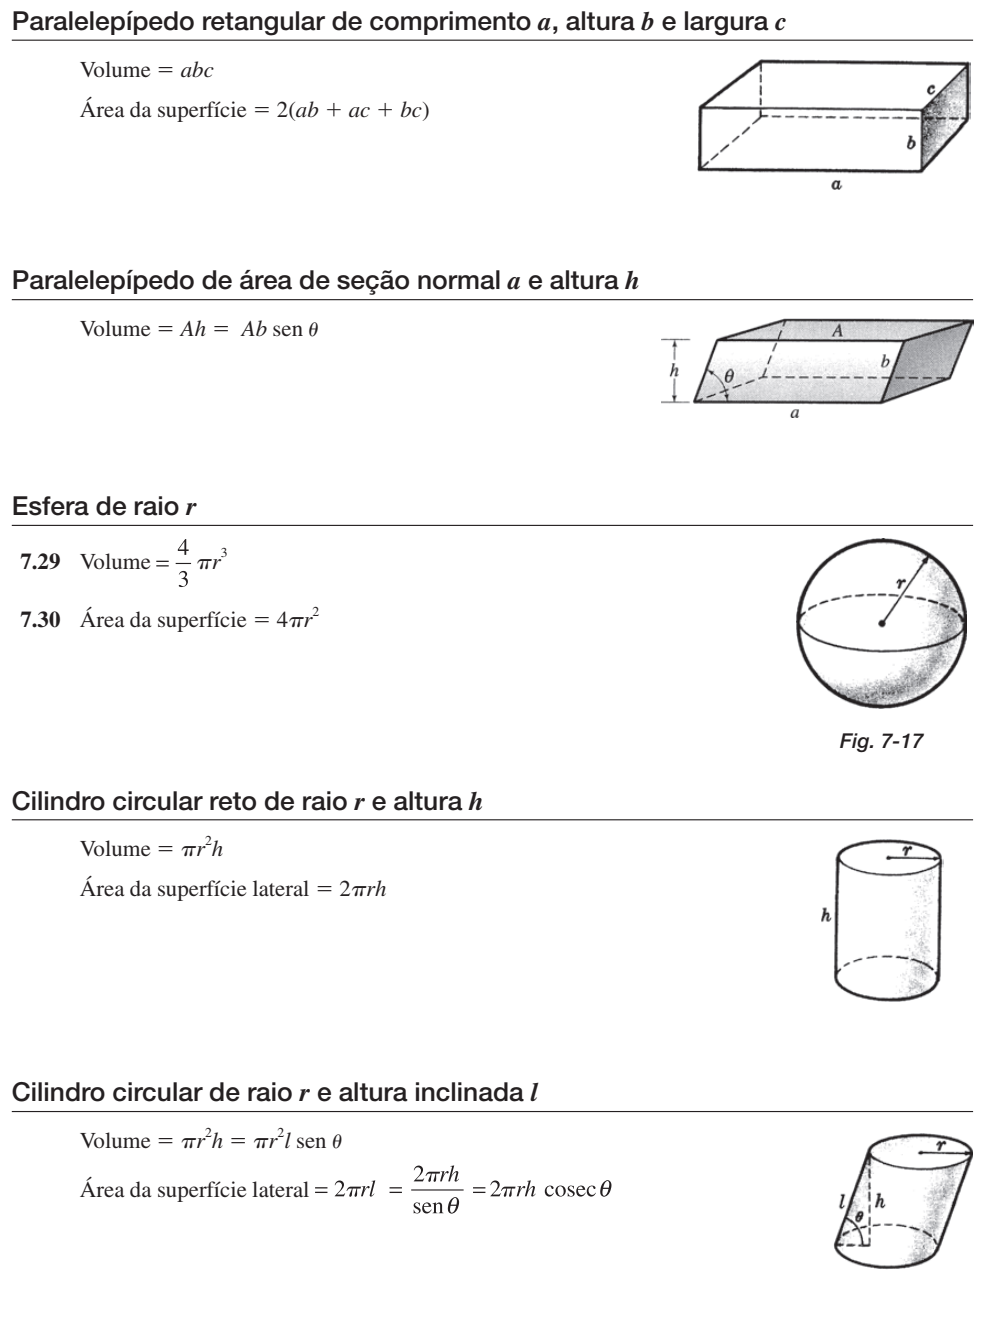
\includegraphics[width=\textwidth]{matematica/geometria/formulas4}
\end{figure}

\begin{figure}[H]
    \centering
    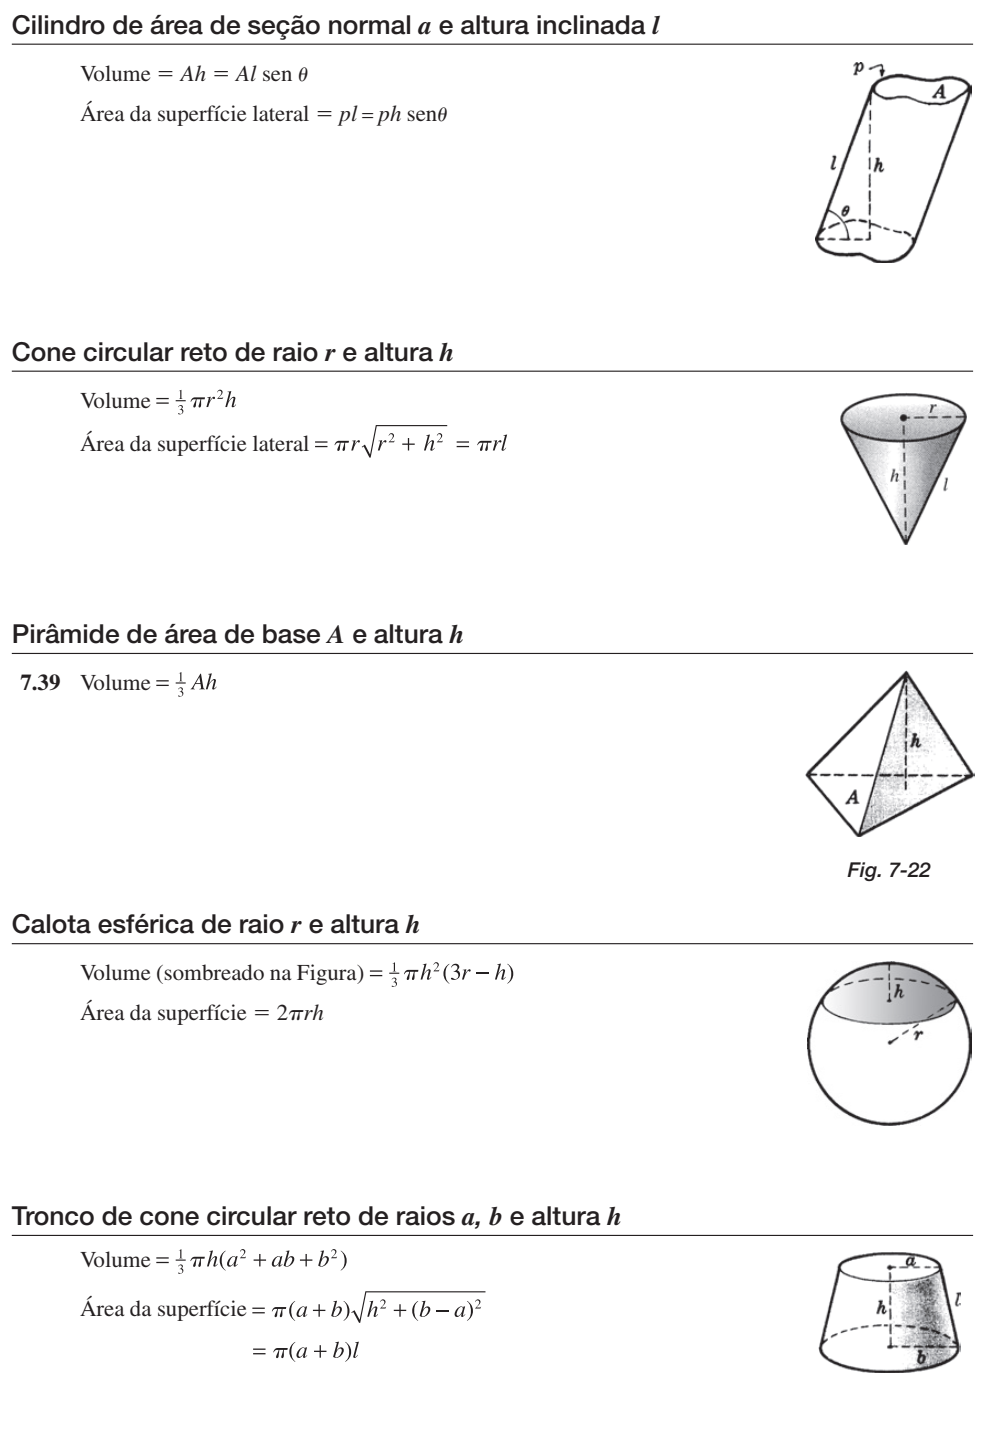
\includegraphics[width=\textwidth]{matematica/geometria/formulas5}
\end{figure}

\begin{figure}[H]
    \centering
    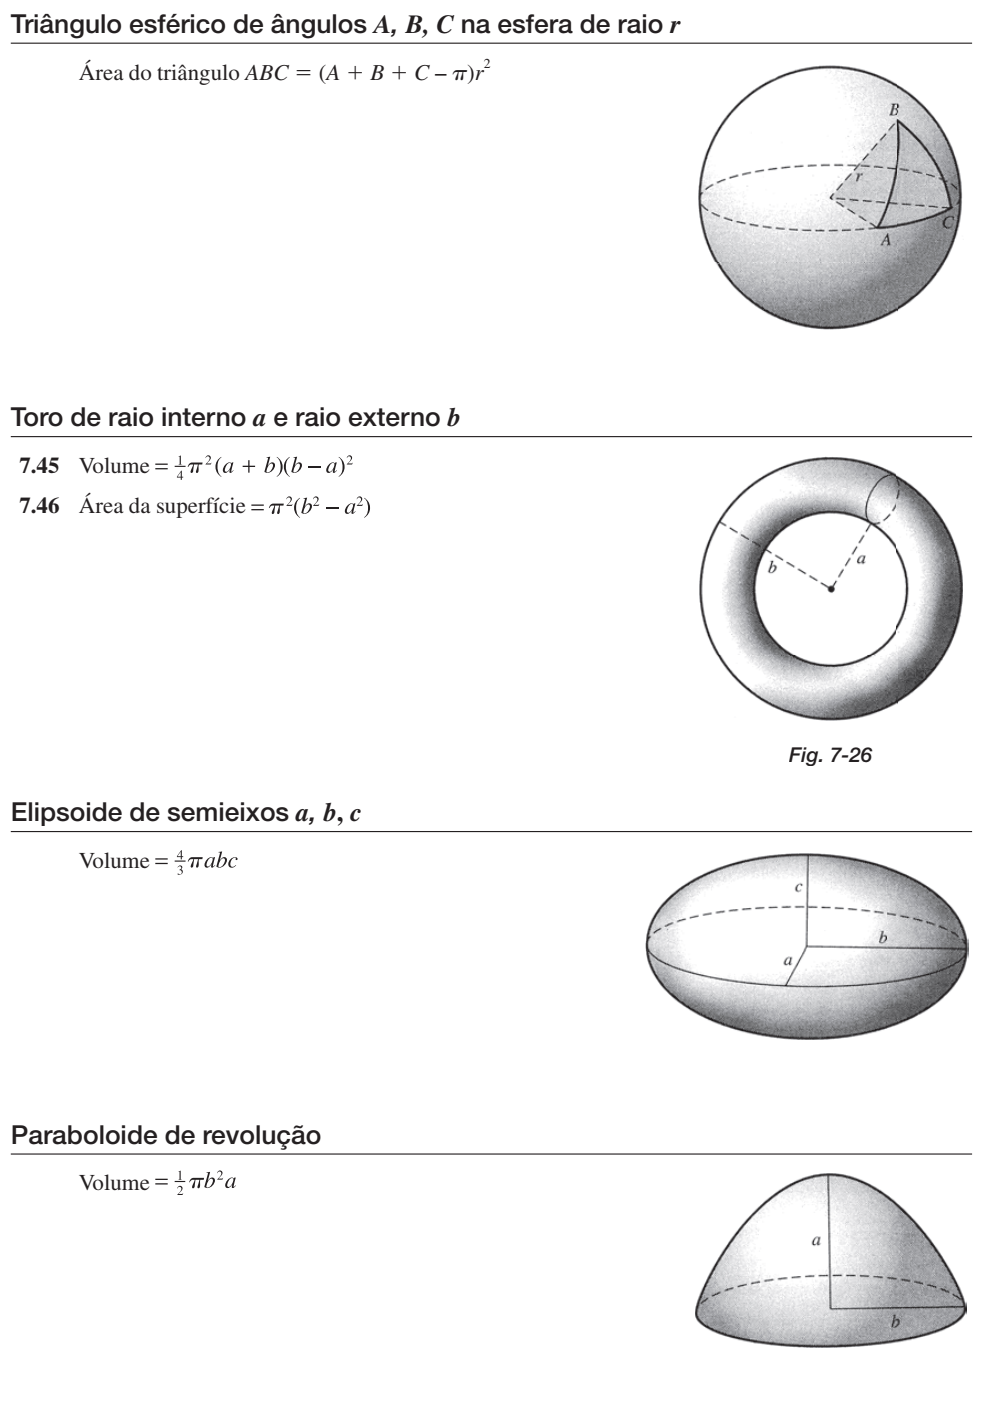
\includegraphics[width=\textwidth]{matematica/geometria/formulas6}
\end{figure}